
\documentclass[hyperref={bookmarks=false}]{beamer}

\useoutertheme{infolines}
\setbeamertemplate{headline}{} % removes the headline that infolines inserts
% \setbeamertemplate{footline}{
%   \hfill%
%   \usebeamercolor[fg]{page number in head/foot}%
%   \usebeamerfont{page number in head/foot}%
%   \insertpagenumber\,/\,\insertpresentationendpage\kern1em\vskip2pt%
% }
\setbeamertemplate{footline}{
  \hfill%
  \usebeamercolor[fg]{page number in head/foot}%
  \usebeamerfont{page number in head/foot}%
  \insertpagenumber\kern1em\vskip2pt%
}
\setbeamertemplate{navigation symbols}{}

\usepackage[parfill]{parskip}
\usepackage{color}
\usepackage{listings}
\usepackage{textcomp}
\usepackage[linewidth=0.5pt]{mdframed}
\usepackage{hyperref}
\usepackage{ulem}
\usepackage{tikz}
\normalem
\hypersetup{pdfauthor={Eugene Burmako},pdfsubject={Metaprogramming with Macros},pdftitle={Metaprogramming with Macros}}
\title{Scala Macros}

\lstset{frame=tb,
  aboveskip=3mm,
  belowskip=3mm,
  showstringspaces=false,
  columns=flexible,
  basicstyle={\small\ttfamily},
  numbers=none,
  numberstyle=\tiny\color{0.5,0.5,0.5},
  keywordstyle=\color{blue},
  commentstyle=\color{0,0.6,0},
  stringstyle=\color{0.58,0,0.82},
  frame=single,
  breaklines=true,
  breakatwhitespace=true
  tabsize=3
}

\setbeamercolor{alerted text}{fg=blue}
\setbeamerfont{alerted text}{series=\bfseries,family=\ttfamily}

\newmdenv[innerleftmargin=1mm, innerrightmargin=1mm, innertopmargin=-1mm, innerbottommargin=2mm, leftmargin=-1mm, rightmargin=-1mm]{lstlistinglike}

\AtBeginSection[]
{
  \begin{frame}
    \frametitle{Outline}
    \tableofcontents[currentsection]
  \end{frame}
}

\begin{document}

\title{Metaprogramming with Macros}
\author{Eugene Burmako}
\institute{\'Ecole Polytechnique F\'ed\'erale de Lausanne \\
           \texttt{http://scalamacros.org/}}
\date{10 September 2012}
{
\setbeamertemplate{footline}{}
\begin{frame}
  \titlepage
\end{frame}
}

\begin{frame}[fragile]
\frametitle{The essence of macros}
Macros are programmable code transformers
\end{frame}

\begin{frame}[fragile]
\frametitle{Example} % \only<1>

\begin{lstlistinglike}
\begin{semiverbatim}
(\alert{defmacro} let args
  (cons
   (cons 'lambda
         (cons (map car (car args))
               (cdr args)))
   (map cadr (car args))))
\end{semiverbatim}
\end{lstlistinglike}

Here we declare \emph{let}, a Lisp function. Since it is declared as a macro,
it's automatically plugged into the Lisp evaluator.

We can say that the evaluator installs a macro transformer implemented by the body of the macro
into a slot named \emph{let}.
\end{frame}

\begin{frame}[fragile]
\frametitle{Example} % \only<2>

\begin{lstlistinglike}
\begin{semiverbatim}
(defmacro \text{\color{blue}{let}} \text{\color{violet}{args}}
  (cons
   (cons 'lambda
         (cons (map car (car args))
               (cdr args)))
   (map cadr (car args))))

(\text{\color{blue}{let}} \text{\color{violet}{((x 40) (y 2)) (print (+ x y))}})
\end{semiverbatim}
\end{lstlistinglike}

When the evaluator encounters a form that is an application of \emph{let},
it yields control to the corresponding macro transformer,
passing it the tail of the form.
\end{frame}

\begin{frame}[fragile]
\frametitle{Example} % \only<3>

\begin{lstlistinglike}
\begin{semiverbatim}
(defmacro let args
  (cons
   (cons \text{\color{blue}{'lambda}}
         (cons \text{\color{red}{(map car (car args))}}
               \text{\color{violet}{(cdr args)}}))
   \text{\color{teal}{(map cadr (car args))}}))

\sout{(let ((\text{\color{red}{x}} \text{\color{teal}{40}}) (\text{\color{red}{y}} \text{\color{teal}{2}})) \text{\color{violet}{(print (+ x y))}})}

((\text{\color{blue}{lambda}} \text{\color{red}{(x y)}} \text{\color{violet}{(print (+ x y))}}) \text{\color{teal}{(40 2)}})
\end{semiverbatim}
\end{lstlistinglike}

The macro transformer takes the forms passed by the evaluator,
and computes a resulting form (this is called \emph{macro expansion}).

After that the evaluator proceeds with the form produced by macro expansion.
The value of the new form is returned as the value of the original form.
\end{frame}

\begin{frame}[fragile]
\frametitle{Use cases}

\begin{itemize}
\item Deeply embedded DSLs (database access, testing)
\item Optimization (programmable inlining, fusion)
\item Analysis (integrated proof-checker)
\item Effects (effect containment and propagation)
\end{itemize}

\vskip15pt

\only<2>{Actually these use cases come from our experience with macros in Scala,
which we developed this year.

All the aforementioned scenarios are either already supported by Scala macros
or will be supported in vNext!}
\end{frame}

\begin{frame}[fragile]
\frametitle{Setting the stage}

In this talk we'll be looking into macros for compiled programming languages,
i.e. macros as extensions to compilers.

Different combinations of junction points (function applications, code annotations, custom grammar rules, etc)
and tightness of the integration (parser, namer, typer, etc) produce different challenges.

Today we're going to focus on a particular challenge in macrology: tackling syntactic abstractions.
These slides discuss the ways to represent, analyze and generate code.
\end{frame}

\section{Challenges in macrology: notation}

\begin{frame}[fragile]
\frametitle{Revisiting \emph{let}}

\begin{lstlistinglike}
\begin{semiverbatim}
(defmacro let args
  (cons
   (cons \text{\color{blue}{'lambda}}
         (cons \text{\color{red}{(map car (car args))}}
               \text{\color{violet}{(cdr args)}}))
   \text{\color{teal}{(map cadr (car args))}}))

(let ((\text{\color{red}{x}} \text{\color{teal}{40}}) (\text{\color{red}{y}} \text{\color{teal}{2}})) \text{\color{violet}{(print (+ x y))}})

((\text{\color{blue}{lambda}} \text{\color{red}{(x y)}} \text{\color{violet}{(print (+ x y))}}) \text{\color{teal}{(40 2)}})
\end{semiverbatim}
\end{lstlistinglike}

The code here is quite impenetrable.
Without color coding it would be hard to understand the supposed structure of input and output.
\end{frame}

\begin{frame}[fragile]
\frametitle{Improving \emph{let}}

\setbeamercolor{alerted text}{fg=blue} % maybe fg=red?
\begin{lstlistinglike}
\begin{semiverbatim}
(defmacro let (decls body)
  \alert{`}((lambda \alert{,}(map car decls) \alert{,}body) \alert{,@}(map cadr decls)))

(let ((x 40) (y 2)) (print (+ x y)))

((lambda (x y) (print (+ x y))) (40 2))
\end{semiverbatim}
\end{lstlistinglike}
\setbeamercolor{alerted text}{fg=blue}

This snippet represents a shift towards declarativeness.
Arguments of let are now pattern-matched in the macro signature.
The shape of resulting form is encoded in a template.

Backquote, the template-building operator, is called \emph{quasiquote}.
By default code inside the quasiquote is not evaluated and is copied into the output verbatim
(note that we no longer have to quote \texttt{lambda}).

Comma and comma-at are called \emph{unquote} operators.
They temporarily cancel the effect of quasiquoting, demarcating "holes" in templates.
\end{frame}

\begin{frame}[fragile]
\frametitle{Pushing the envelope}

\setbeamercolor{alerted text}{fg=blue} % maybe fg=red?
\begin{lstlistinglike}
\begin{semiverbatim}
(define-syntax let
  (syntax-rules ()
    ((let ((name expr) ...) body ...)
     ((lambda (name ...) body ...) expr ...))))

(let ((x 40) (y 2)) (print (+ x y)))

((lambda (x y) (print (+ x y))) (40 2))
\end{semiverbatim}
\end{lstlistinglike}
\setbeamercolor{alerted text}{fg=blue}

This amazing notation comes from Scheme and is dubbed \emph{macro by example} (MBE).
With the ellipsis operator it naturally captures repetitions in the input form
and translates them into the output.

\texttt{syntax-rules} is a shortcut that eliminates the syntactic overhead of quasiquoting at a cost
of supporting unquotes only for variables bound in a match. However MBE per se doesn't prevent
arbitrary unquoting. \texttt{syntax-case}, a low-level implementation of MBE, supports all the
functionality provided by quasiquotes.
\end{frame}

\begin{frame}[fragile]
\frametitle{Typechecking quasiquotes: strict}

\begin{lstlistinglike}
\begin{semiverbatim}
-| fun plus x = <fn y => ~x + y>;
val plus = Fn : <int> -> <int -> int>

-| val w = <fn y => ~(plus <y>)>;
val w = <(fn a => (fn b => a \%+ b))> : <int -> int -> int>
\end{semiverbatim}
\end{lstlistinglike}

MetaML is a statically typechecked language with quasiquotes. Its typesystem guarantees that
if a meta-program is well-typed then all possibly produced object-programs will be well-typed as well.

Unlike in lisps, quasiquotes in MetaML cannot have unbound free variables, which effectively means
that meta-programs cannot introduce new bindings (e.g. it's not possible to express \emph{let} as a macro).
This is a sacrifice to the altar of strong type safety guarantees.
\end{frame}

\begin{frame}[fragile]
\frametitle{Typechecking quasiquotes: strict}

\begin{lstlistinglike}
\begin{semiverbatim}
mac (let seq x = e1 in e2 end) =
   \$(let val x = ?e1 in ?e2 end)
\end{semiverbatim}
\end{lstlistinglike}

MacroML is a macro system built on top of MetaML. It inherits typing discipline of its parents,
but introduces a clever way to create certain bindings without compomising type safety.

In the example above \texttt{\$} stands for "delay" and \texttt{?} stands for "force". Macro \texttt{seq}
implements (wtf does it implement?).

To typecheck the fluent binding to \texttt{x}, MacroML tracks the name of the bindee parameter in the type
of the body parameters such as \texttt{e}i.
\end{frame}

\begin{frame}[fragile]
\frametitle{Typechecking quasiquotes: lenient}

\begin{lstlistinglike}
\begin{semiverbatim}
macro using(name, expr, body) \{
  <[
    def \$name = \$expr;
    try \{ \$body \} finally \{ \$name.Dispose() \}
  ]>
\}

using(db, Database("localhost"), db.LoadData())
\end{semiverbatim}
\end{lstlistinglike}

Nemerle allows quasiquotes to contain free variables, it even permits
splicing into binding positions (like in \texttt{def \$name = \$expr}).

This makes it impossible to typecheck quasiquotes at their declaration site,
but the result of macro expansion that uses such quasiquotes is typechecked anyways,
so errors are still caught at compile-time.

Relaxed typechecking rules like in Nemerle have proven to be essential
for a practical metaprogramming system.
\end{frame}

\begin{frame}[fragile]
\frametitle{Typechecking quasiquotes: the best of both worlds}

The ideal typechecking discipline would allow programmers to freely mix
typed and untyped quasiquotes.

In F\# both quasiquoting (\texttt{<@...@>}) and splicing (\texttt{\%}) operators
have untyped versions (\texttt{<@@...@@>} and \texttt{\%\%} respectively).

Unfortunately they are only untyped in a sense that untyped splicing
allows \texttt{Expr} instead of \texttt{Expr<'a>}. Untyped quasiquotes do perform typechecking
using type inference to determine type bounds for holes, which are verified at runtime.
As a result, \texttt{<@@ (\%\%x).Name @@>} won't typecheck, whereas \texttt{<@@ (\%\%x).ToString() @@>}
will fail at runtime.

In a 15 year old paper, Mark Shields, Tim Sheard and Simon Peyton Jones propose a type system
that can defer type inference to runtime. Their findings can probably be adapted to the task at hand.
\end{frame}

\section{Challenges in macrology: bindings}

\begin{frame}[fragile]
\frametitle{Motivating example}

\begin{lstlistinglike}
\begin{semiverbatim}
(defmacro or (x y)
  `(let ((t ,x))
     (if t t ,y)))

(or 42 "strange")
\end{semiverbatim}
\end{lstlistinglike}

One of the appealing features of macros is their ability to
control evaluation order. For example, it's possible to write
a short-circuiting \texttt{or} macro.

In this example, however, I would like to highlight the temporary variable
that had to be introduced in order to prevent double evaluation.

The implementation is very simple. Yet it has two mistakes
that can lead to subtle bugs. Let's take a closer look.
\end{frame}

\begin{frame}[fragile]
\frametitle{Mistake \#1}

\begin{lstlistinglike}
\begin{semiverbatim}
(defmacro or (x y)
  `(let ((t ,x))
     (if t t ,y)))

(let ((t \#t))
  (or \#f t))
\end{semiverbatim}
\end{lstlistinglike}

The first bug manifests itself when there's a variable named \texttt{t} at the call site,
and it's used in the second argument of the \texttt{or} macro. We can say that a variable introduced during macro expansion shadows a binding from the macro use site.
\end{frame}

\begin{frame}[fragile]
\frametitle{Hygiene}

\begin{quote}
Hygiene Condition for Macro Expansion.

Generated identifiers that become binding instances in
the completely expanded program must only bind variables
that are generated at the same transcription step.
\end{quote}

\begin{flushright}
\textemdash Eugene Kohlbecker\\
PhD Thesis
\end{flushright}
\end{frame}

\begin{frame}[fragile]
\frametitle{Breaking hygiene}

\begin{lstlistinglike}
\begin{semiverbatim}
(define-syntax forever
  (syntax-rules ()
    ((forever body ...)
     (call/cc (lambda (abort)
                (let loop () body ... (loop)))))))

(forever (print 4) (print 2) (abort))
\end{semiverbatim}
\end{lstlistinglike}

At times, though, it's useful to break hygiene and meld lexical contexts
from different transcription steps.

We've seen one such example, when studying the \texttt{using} macro written in Nemerle.
Here's another one that features a DSL for writing loops. Whenever we're inside a loop
introduced by our DSL, we should be able to use \texttt{abort} to quit.

For this snippet to work, the binding created by \texttt{forever} must be non-hygienic,
since \texttt{abort} is supposed to be accessible from \texttt{body}.
\end{frame}

\begin{frame}[fragile]
\frametitle{Mistake \#2}

\begin{lstlistinglike}
\begin{semiverbatim}
(defmacro or (x y)
  `(let ((t ,x))
     (if t t ,y)))

(let ((let print))
  (or \#f \#t))
\end{semiverbatim}
\end{lstlistinglike}

The second bug is, in a sense, dual to the first one. Previously, a binding introduced by a macro
interfered with a binding at the macro use site. Now a binding introduced at the call site destroys
a binding at the macro definition site.
\end{frame}

\begin{frame}[fragile]
\frametitle{Referential transparency}

\begin{quote}
Macros defined in the high-level specification language are referentially
transparent in the sense that a macro-introduced identifier refers to the
binding lexically visible where the macro definition appears rather than to
the top-level binding or to the binding visible where the macro call appears.
\end{quote}

\begin{flushright}
\textemdash Kent Dybvig et al.\\
Syntactic Abstractions in Scheme
\end{flushright}
\end{frame}

\begin{frame}[fragile]
\frametitle{State of the art}

\begin{itemize}
\item Typical approaches to fixing the aforementioned problems
are alpha-renaming and gensymming (from \texttt{gensym}).
\item There are frameworks that provide hygiene and referential transparency automatically.
Scheme is especially famous for pushing this research.
\item These automatic frameworks usually have enough flexibility to allow for
the use cases that require non-hygienic bindings.
\end{itemize}

\end{frame}

\section{Macros in Template Haskell}

\begin{frame}[fragile]
\frametitle{\texttt{printf}}

\begin{lstlistinglike}
\begin{semiverbatim}
\alert<1>{printf :: String -> \alert<2>{Expr}}
printf s = gen (parse s) \alert<2>{[|} "" \alert<2>{|]}

gen :: [Format] -> Expr -> Expr
gen [] x = x
gen (D : xs) x = \alert<2>{[|} \only<1-2,4->{\\n}\only<3>{\text{\color{violet}{\\n}}} -> \alert<2>{\$(}gen xs \alert<2>{[|} \alert<2>{\$}x \alert<3>{++} show \only<1-2,4->{n}\only<3>{\text{\color{violet}{n}}} \alert<2>{|]}\alert<2>{)} \alert<2>{|]}
gen (S : xs) x = \alert<2>{[|} \only<1-2,4->{\\s}\only<3>{\text{\color{red}{\\s}}} -> \alert<2>{\$(}gen xs \alert<2>{[|} \alert<2>{\$}x \alert<3>{++} \only<1-2,4->{s}\only<3>{\text{\color{red}{s}}} \alert<2>{|]}\alert<2>{)} \alert<2>{|]}
gen (L s : xs) x = gen xs \alert<2>{[|} \alert<2>{\$}x \alert<3>{++} \alert<2>{\$(}\alert<4>{lift s}\alert<2>{)} \alert<2>{|]}

\only<1,3->{\alert<1>{\$(}}\only<2>{\text{\color{teal}{\$(}}}printf "\alert<4>{Error:} %s\alert<4>{ on line }%d"\only<1,3->{\alert<1>{)}}\only<2>{\text{\color{teal}{)}}} msg line

(\only<1-2,4->{\\s0}\only<3>{\text{\color{red}{\\s0}}} -> \only<1-2,4->{\\n1}\only<3>{\text{\color{violet}{\\n1}}} ->
  \alert<4>{"Error: "} \alert<3>{++} \only<1-2,4->{s0}\only<3>{\text{\color{red}{s0}}} \alert<3>{++} \alert<4>{" on line "} \alert<3>{++} show \only<1-2,4->{n1}\only<3>{\text{\color{violet}{n1}}})
\end{semiverbatim}
\end{lstlistinglike}

\only<1>{In Template Haskell macros don't need a special declaration form
(unlike in Lisp, they are first-class),
at a cost of requiring an explicit trigger for macro expansion.}

\only<2>{Template Haskell has the notion of quasiquoting and unquoting (called \emph{splicing}
in authors' terms). Splicing outside quasiquotes (or an explicit call to \texttt{splice}) triggers macro expansion.}

\only<3>{Quasiquotes automatically alpha-rename introduced identifiers to ensure hygiene.
Template Haskell also solves the referential transparency problem by implementing cross-stage persistence
for static symbols.}

\only<4>{For non-static symbols, general case of cross-stage persistence is undecidable.
However if the programmer knows how to reproduce a certain datum at runtime, he implements
the \texttt{Lift} typeclass and calls \texttt{lift}.}
\end{frame}

\begin{frame}[fragile]
\frametitle{Bindings}

\begin{lstlistinglike}
\begin{semiverbatim}
cross2a :: Expr -> Expr -> Expr
cross2a f g = [| \\(x,y) -> (\$f x, \$g y) |]

cross2c :: Expr -> Expr -> Expr
cross2c f g =
  do \{ x <- gensym "x"
     ; y <- gensym "y"
     ; ft <- f
     ; gt <- g
     ; return (Lam [Ptup [Pvar x, Pvar y]]
                   (Tup  [App ft (Var x)
                         ,App gt (Var y)]))
     \}
\end{semiverbatim}
\end{lstlistinglike}

At the low level of Template Haskell lie plain ADTs that represent program fragments.
Quotation monad can make low-level ASTs hygienic (but also may ignore hygiene).
High level of syntactic abstraction is represented by quasiquotes, which translate to
the hygienic quotation monad.
\end{frame}

\begin{frame}[fragile]
\frametitle{Typechecking}

\begin{itemize}
\item Quasiquotes are expanded in \emph{re}namer (later in the pipeline bindings are frozen),
and they must not contain unbound free symbols.
\item Every quotation is then sanity-checked in typer to reject nonsense like \texttt{[| "hello" \&\& True |]}.
Having passed the check, quotations pass the type check and are assigned the \texttt{Q Exp} type.
\item After quotations are typechecked, macros are expanded, and the compilation goes on just
as if the programmer had written the expanded program in the first place.
\end{itemize}

A retrospective write-up from TH developers indicates that:
\begin{itemize}
\item There is a real need for strongly typed quotes \texttt{TExp a} (for more robustness).
\item Normal quotes shouldn't be typechecked at all (to allow for more flexibility, with an important
particular case of splicing into binding positions).
\end{itemize}
\end{frame}

\section{Macros in Nemerle}

\begin{frame}[fragile]
\frametitle{Overview}

\begin{lstlistinglike}
\begin{semiverbatim}
\alert<1>{macro} identity(\only<1>{e}\only<2>{\text{\color{teal}{e}}}) \{
  <[ def \only<1>{f}\only<2>{\text{\color{red}{f}}}(\only<1>{x}\only<2>{\text{\color{blue}{x}}}) \{ \only<1>{x}\only<2>{\text{\color{blue}{x}}} \}; \only<1>{f}\only<2>{\text{\color{red}{f}}}(\$\only<1>{e}\only<2>{\text{\color{teal}{e}}}) ]>
\}

identity\alert<1>{(}\only<1>{f(1)}\only<2>{\text{\color{teal}{f(1)}}}\alert<1>{)}

\{
  def \only<1>{f_42}\only<2>{\text{\color{red}{f_42}}}(\only<1>{x_43}\only<2>{\text{\color{blue}{x_43}}}) \{ \only<1>{x_43}\only<2>{\text{\color{blue}{x_43}}} \};
  \only<1>{f_42}\only<2>{\text{\color{red}{f_42}}}(\only<1>{f(1)}\only<2>{\text{\color{teal}{f(1)}}})
\}
\end{semiverbatim}
\end{lstlistinglike}

\only<1>{Macros in Nemerle are Lisp-like in a sense that they are second-class, but
are transparent to the user.

Unlike Lisp, Nemerle is statically typed and has rich syntax.
Macros provide extension points to both of these aspects.
They can change syntax and control typechecking (alas, outside the scope of this talk).}

\only<2>{Nemerle has quasiquotes and unquotes (called \emph{splices} like in Template Haskell).
They provide automatic alpha-renaming to preserve hygiene.
Cross-stage persistence is only supported for static symbols.}
\end{frame}

\begin{frame}[fragile]
\frametitle{Typechecking}

\begin{lstlistinglike}
\begin{semiverbatim}
cache(e: Expr): Expr * Expr \{
  | <[ \$o.\$m ]> => (<[ def tmp = \$o ]>, <[ tmp.\$m ]>)
  | <[ \$o[\$i] ]> => (<[ def (tmp1, tmp2) = (\$o, \$i) ]>,
                     <[ tmp1[tmp2] ]>)
  | _ => (<[ () ]>, e)
\}
\end{semiverbatim}
\end{lstlistinglike}

Designers of Nemerle were aware of the "too strongly typed" problem of quasiquotes
in Template Haskell, so they decided not to typecheck them before they are used
in macro expansions.

In fact they went even further - quasiquotes are not only untyped, but they also
don't get their free variables resolved until being used (with an exception for
references to static symbols). This defies one of the aspects of referential transparency,
but in return provides flexibility, e.g. splicing into binding positions at zero implementation cost.
\end{frame}

\begin{frame}[fragile]
\frametitle{Hygiene}

\only<1>{Nemerle assigns colors to every identifier in the program.}

\only<2->{
\vskip15pt
\begin{figure}
\centering
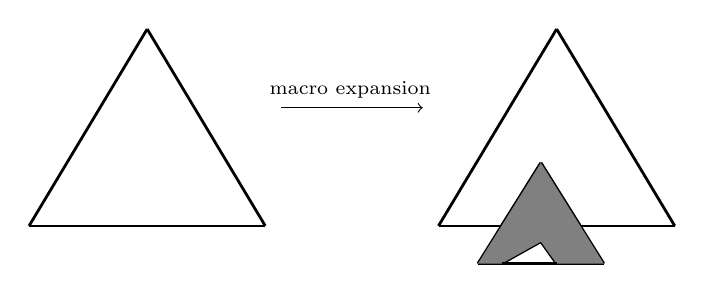
\begin{tikzpicture}
\draw[line width=1pt] (0.0, 0.0) -- (1.5, 2.5);
\draw[line width=1pt] (3.0, 0.0) -- (1.5, 2.5);
\draw[line width=1pt] (0.0, 0.0) -- (3.0, 0.0);
\draw [->] (3.2, 1.5) -- (5.0, 1.5) node[pos=-0.15, above right] {\scriptsize{macro expansion}};
\draw[line width=1pt] (5.2, 0.0) -- (6.7, 2.5);
\draw[line width=1pt] (8.2, 0.0) -- (6.7, 2.5);
\draw[line width=1pt] (5.2, 0.0) -- (6.0, 0.0);
\draw[line width=1pt] (6.0, 0.0) -- (6.5, 0.8);
\draw[line width=1pt] (6.5, 0.8) -- (7.0, 0.0);
\draw[line width=1pt] (7.0, 0.0) -- (8.2, 0.0);
%%------------
\draw[line width=1pt] (6.5, 0.8) -- (5.7, -0.48);
\draw[line width=1pt] (6.5, 0.8) -- (7.3, -0.48);
\draw[line width=1pt] (5.7, -0.48) -- (6.0, -0.48);
\draw[line width=1pt] (6.7, -0.48) -- (7.3, -0.48);
\draw[line width=1pt] (6.0, -0.48) -- (6.5, -0.2);
\draw[line width=1pt] (6.7, -0.48) -- (6.5, -0.2);
\path[fill=gray] (6.5, 0.8) -- (5.7, -0.48) -- (6.0, -0.48) -- (6.5, -0.2) -- (6.7, -0.48) -- (7.3, -0.48) -- cycle;
%%------------
\draw[line width=1pt] (6.0, -0.48) -- (6.7, -0.48);
\end{tikzpicture}
\end{figure}
\vskip15pt}

\only<2>{Given \texttt{u}, the color of the use site, and \texttt{m}, a fresh color
assigned to the current macro expansion:
\begin{itemize}
\item Most identifiers introduced in that expansion get colored with \texttt{m}
\item Macro arguments and \texttt{\$(name:\ usesite)} splices get colored with \texttt{u}
\item \texttt{\$(name:\ dyn)} splices become polychromatic
\item Colors can also be tinkered with manually
\end{itemize}
}

\only<3>{After all colors are resolved it is easy to bind identifiers:
\begin{itemize}
\item Use refers to the nearest preceding declaration of the matching color
(polychromatics match any color, others only match their own)
\item Unbound identifiers are looked up in global scope.
\end{itemize}}

\end{frame}

\section{Macros in Racket}

\section{Our research}

\begin{frame}[fragile]
\frametitle{Questions}
\begin{enumerate}
\item Is it ok to copy/paste snippets and drawings from the papers being studied?
\item Examples. Are they any good?
\item Minimal volume of the write-up?
\end{enumerate}
\end{frame}

\end{document}